\documentclass[11pt,a4paper]{article}
\usepackage[T1]{fontenc}
\usepackage[utf8]{inputenc}
\usepackage{lmodern}
\usepackage[margin=2.3cm]{geometry}
\usepackage{booktabs}
\usepackage{tabularx}
\usepackage{longtable}
\usepackage{array}
\usepackage[table,dvipsnames]{xcolor}
\usepackage{graphicx}
\usepackage{float}
\usepackage{enumitem}
\usepackage{titlesec}
\usepackage{parskip}
\usepackage{setspace}
\usepackage{needspace}
\usepackage[hidelinks]{hyperref}

\setstretch{1.2}
\setlength{\parskip}{0.7em}
\setlist{itemsep=0.3em, topsep=0.3em}
\renewcommand{\arraystretch}{1.35}
\definecolor{accent}{RGB}{31,78,95}
\definecolor{ok}{RGB}{21,128,61}
\definecolor{part}{RGB}{180,83,9}
\definecolor{no}{RGB}{185,28,28}
\titleformat{\section}{\Large\bfseries\color{accent}}{\thesection}{0.8em}{}
\titleformat{\subsection}{\large\bfseries}{\thesubsection}{0.8em}{}
\titlespacing*{\section}{0pt}{1.6em}{0.7em}
\titlespacing*{\subsection}{0pt}{1.1em}{0.4em}
\newcolumntype{L}{>{\raggedright\arraybackslash}X}
\newcolumntype{P}[1]{>{\raggedright\arraybackslash}p{#1}}
\newcommand{\file}[1]{\texttt{\small #1}}
\newcommand{\MET}{\textcolor{ok}{\textbf{Met}}}
\newcommand{\PART}{\textcolor{part}{\textbf{Partly}}}
\newcommand{\NOT}{\textcolor{no}{\textbf{Not yet}}}
\newcommand{\dep}{\rowcolor{gray!18}}
\newcommand{\answer}[1]{\par\noindent\colorbox{accent!8}{\parbox{\dimexpr\linewidth-2\fboxsep}{\vspace{0.4em}\textbf{Answer.} #1\vspace{0.4em}}}\par}

\begin{document}

\begin{titlepage}
\centering
\vspace*{4.5cm}
{\Huge\bfseries\color{accent} TinyIDS\par}
\vspace{1em}
{\LARGE Lightweight, explainable intrusion detection for IoT gateways\par}
\vspace{2em}
{\Large Results against the project proposal\par}
\vspace{1.5em}
{\large RQ1--RQ3, objectives, targets and deliverables\par}
\vfill
{\large Department of Information Technology, IIIT Allahabad \\ November 2026\par}
\vspace{1.5cm}
\end{titlepage}

\tableofcontents
\vspace{1em}
\noindent\colorbox{gray!18}{\strut\ Grey rows\ } = the model deployed on the Raspberry Pi
(LightGBM, 3 classes, 14 features, 974 KB).

\newpage
% =====================================================================================================
\section{At a glance}

\subsection{The deployed system}

One LightGBM model on a Raspberry Pi 4 gateway classifies every window of 10 packets from a sender as
\textbf{Benign}, \textbf{Flood} or \textbf{Recon}, using 14 features (packet sizes, TCP flags, protocol). Rules cover
what one window cannot show (DoS vs DDoS, port scans, MQTT brute force, spoofing). Every alert carries its top-3
TreeSHAP reasons; attackers are blocked by the Pi's firewall (iptables).

\begin{figure}[H]
\centering
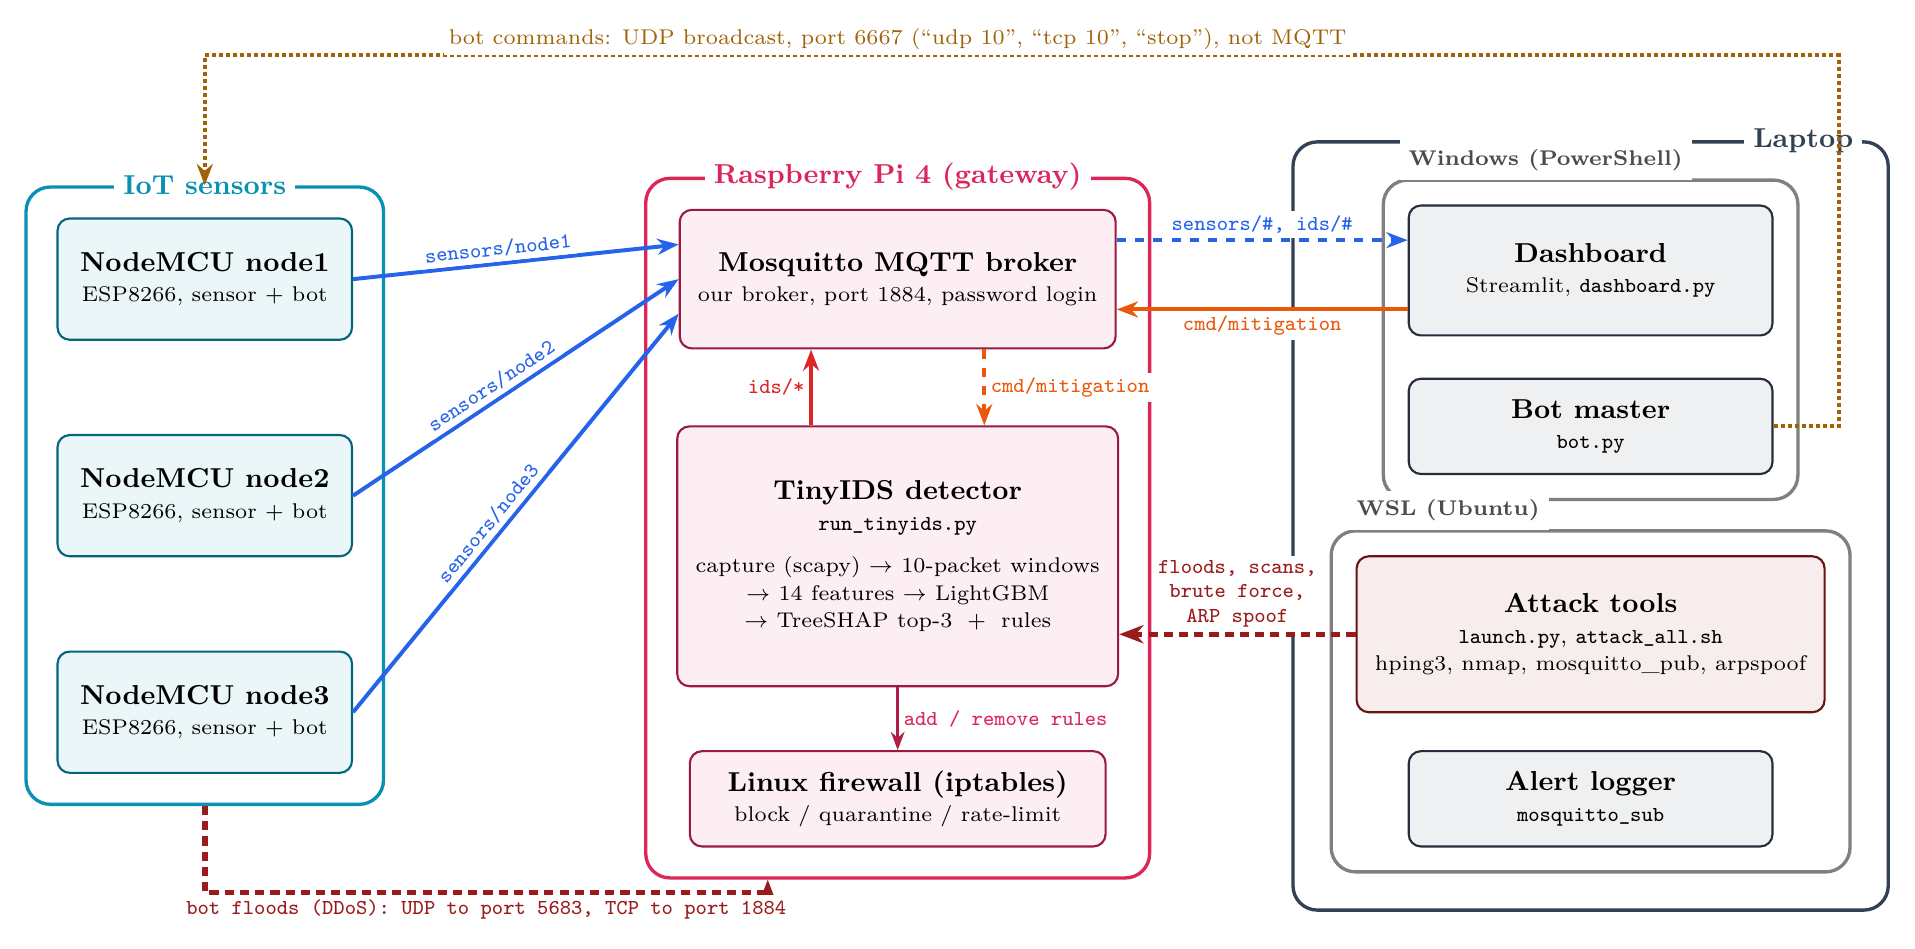
\includegraphics[width=\linewidth]{../ppts/assets/hld.png}
\caption{High-level design: 3 NodeMCU sensors, the Raspberry Pi gateway (broker, detector, firewall), the laptop
(dashboard, bot master, attack tools).}
\end{figure}

\subsection{Evaluation targets (proposal, ``Evaluation metrics'')}

\begin{center}
\begin{tabularx}{\linewidth}{P{3.2cm}P{3.4cm}LP{1.6cm}}
\toprule
Metric & Target & Result (deployed model) & Status \\
\midrule
\dep Binary F1 & $\geq$ 0.98 & \textbf{0.997} on 973,829 CICIoT2023 test rows & \MET \\
\dep False-positive rate & reported & 0.97\% (dataset); \textbf{0 false alarms} on 3 NodeMCUs live & \MET \\
8-class macro-F1 & within 2\% of full model & full 45 features: 0.705; within 2\% needs 30 features (RQ1) & \MET \\
\dep Model size & $<$ 1 MB & \textbf{974 KB} & \MET \\
\dep Peak RAM on Pi & $<$ 100 MB & \textbf{77--78 MB} (whole detector, under attack) & \MET \\
\dep Latency & $<$ 5 ms per flow & \textbf{0.7--1.4 ms} per window on the Pi & \MET \\
\dep Throughput & $\geq$ 500 flows/s & $\approx$ 700--1,400 windows/s (from the latency; not measured on its own) & \PART \\
Energy & mJ per inference & not measured (no USB power meter) & \NOT \\
\dep SHAP latency & $<$ 50 ms per alert & \textbf{5--14 ms} on the Pi & \MET \\
\bottomrule
\end{tabularx}
\end{center}

% =====================================================================================================
\section{Research questions}

\subsection{RQ1: How few features keep macro-F1 within 2\% of the full-feature model?}

SHAP ranking (mean $|$SHAP$|$) from the full LightGBM, retrain with the top-$k$ features, test on the full
CICIoT2023 test split. IAT is excluded (a capture-time shortcut), so ``full'' = 45 features.

\begin{center}
\begin{tabular}{lccccccc}
\toprule
Task, training data & 5 & 10 & 15 & 20 & 25 & 30 & all 45 \\
\midrule
8-class, 20\% sample & 0.568 & 0.645 & 0.675 & 0.676 & 0.676 & \textbf{0.685} & 0.705 \\
3-class, 20\% sample & 0.807 & 0.863 & \textbf{0.879} & 0.882 & 0.884 & 0.884 & 0.885 \\
3-class, 100\% of rows & 0.836 & \textbf{0.874} & 0.884 & 0.886 & 0.887 & 0.889 & 0.888 \\
\bottomrule
\end{tabular}
\end{center}
{\small Bold = smallest feature count within 0.02 of the all-45 model. 8-class: Benign + 7 attack families.}

\textbf{Deployment constraint.} Only 14 of the 46 features are computed by our gateway exactly as in the dataset
(measured by recording our own floods); the others are computed differently live, are shortcuts, or are constant
for our attacks. Within these 14 Pi-computable features:

\begin{center}
\begin{tabular}{lcccc}
\toprule
Pi-computable features (3-class) & 5 & 7 & 10 & 14 \\
\midrule
Dataset test macro-F1 & 0.646 & 0.722 & \textbf{0.754} & 0.760 \\
\bottomrule
\end{tabular}
\end{center}

\answer{On the dataset, \textbf{30 of 45} features keep the 8-class macro-F1 within 2\% of the full model;
for the 3-class task we deploy, \textbf{15} are enough (\textbf{10} when trained on all rows). On the real gateway
only 14 features can be computed identically, and \textbf{10 of those} stay within 1\% of all 14. The remaining gap
to the 45-feature model is almost entirely the Recon class.}

\begin{figure}[H]
\centering
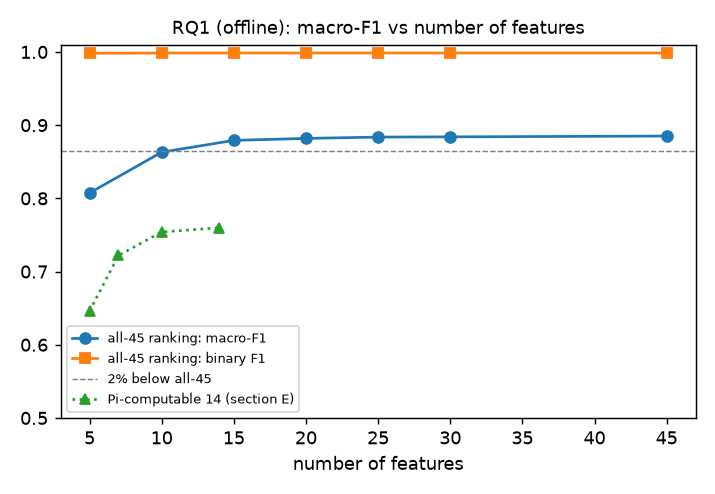
\includegraphics[width=0.62\linewidth]{images/rq1_all45.png}
\caption{RQ1, 3-class task: macro-F1 against the number of features.}
\end{figure}

\subsection{RQ2: Which compressed model gives the best accuracy per millisecond and per megabyte?}

Binary task, 15 SHAP-selected features for trees, 45 for nets; test = full CICIoT2023 test split. Latency = one
window at a time, \textbf{measured on the laptop} (the Pi is about 3--4$\times$ slower).

\begin{center}
\begin{tabular}{llrrr}
\toprule
Model & Compression & Size (KB) & Macro-F1 & Latency (ms) \\
\midrule
LightGBM & original & 6,667 & 0.945 & 0.710 \\
LightGBM & pruned (150 rounds) & 260 & 0.917 & 0.681 \\
LightGBM & pruned $\rightarrow$ ONNX & 157 & 0.917 & 0.019 \\
Random Forest & pruned (30 trees, d 12) $\rightarrow$ ONNX & 859 & 0.909 & 0.012 \\
MLP (3 layers) & ONNX fp32 & 57 & 0.916 & 0.010 \\
MLP (3 layers) & ONNX INT8 (static) & \textbf{19} & 0.915 & 0.012 \\
1D-CNN & ONNX fp32 & 80 & 0.879 & 0.034 \\
1D-CNN & ONNX INT8 (static) & 28 & 0.880 & 0.025 \\
\bottomrule
\end{tabular}
\end{center}

\textbf{Measured on the Pi} (2,000 test windows, one at a time):

\begin{center}
\begin{tabular}{lrrr}
\toprule
LightGBM model & Size & Time per window & SHAP per alert \\
\midrule
Earlier version (2 models) & 1,014 + 7,032 KB & 1.88 ms & 45.65 ms \\
Small version ($<$ 1 MB) & 974 + 776 KB & 1.09 ms & 2.59 ms \\
\dep Deployed (1 model, 3 classes, live) & 974 KB & 0.7--1.4 ms & 5--14 ms \\
\bottomrule
\end{tabular}
\end{center}

\answer{\textbf{Per megabyte:} the INT8 MLP (19 KB, macro-F1 0.915, no accuracy lost to quantization).
\textbf{Per millisecond:} the ONNX models are all fast (0.01--0.03 ms on the laptop). We deploy the
\textbf{pruned LightGBM}: it meets every target on the Pi (974 KB, $\sim$1 ms) and is the only model with
\textbf{exact, fast TreeSHAP} explanations, which the nets cannot give in milliseconds. INT8 made the nets 3$\times$
smaller but not faster for single windows. \emph{Open:} the full RQ2 table (all compressed models) has not yet been
run on the Pi; the benchmark script is ready.}

\subsection{RQ3: Can SHAP explanations be produced on the gateway fast enough for live alerts?}

\begin{center}
\begin{tabular}{lrr}
\toprule
Model on the Raspberry Pi & SHAP per alert & Target \\
\midrule
Earlier, large model (7 MB) & 45.65 ms & $<$ 50 ms \\
Small model & 2.59 ms & $<$ 50 ms \\
\dep Deployed model, live under attack & \textbf{5--14 ms} & $<$ 50 ms \\
\bottomrule
\end{tabular}
\end{center}

\answer{\textbf{Yes.} LightGBM's built-in TreeSHAP (exact, no extra library) gives the top-3 features of every
alert in 5--14 ms on the Pi, 4--10$\times$ under the 50 ms target, and they are shown live on the dashboard
(e.g.\ UDP flood: \file{Protocol Type}, \file{UDP}, \file{Min}). Model size matters: a 7 MB model needed 46 ms,
the $<$ 1 MB one 3 ms.}

% =====================================================================================================
\section{Objectives}

\begin{longtable}{P{5.2cm}P{8.0cm}P{1.6cm}}
\toprule
Objective (proposal) & What was done & Status \\
\midrule
\endhead
1. Benchmark $\geq$ 4 classifiers, binary / 8 / 34-class & RF, LightGBM, MLP, 1D-CNN on all three tasks (Section 4) & \MET \\
2. SHAP-based feature selection & RQ1 (Section 2.1) & \MET \\
3. Compress (pruning, INT8) and deploy on the Pi & pruning + ONNX + INT8 built; pruned LightGBM deployed; Pi
benchmark of all compressed models still to run & \PART \\
4. MQTT testbed with ESP32 nodes, replayed or live attacks & 3 NodeMCU (ESP8266, same family) + Mosquitto on the
Pi; \textbf{live} attacks: floods, scans, brute force, botnet DDoS & \MET \\
5. Dashboard with top contributing features & Streamlit dashboard: alerts with top-3 SHAP, IPS controls & \MET \\
6. 6-page conference paper & -- & \NOT \\
\bottomrule
\end{longtable}

% =====================================================================================================
\section{Objective 1: the four-classifier benchmark}

45 features (IAT excluded), 20\% stratified training sample, scored on the \textbf{full} CICIoT2023 test split
(1.18 M rows). ``Edge'' = the compressed version. Latency = one row on the laptop.

\begin{longtable}{llrrrr}
\toprule
Task & Model & Accuracy & Macro-F1 & Size (KB) & Latency (ms) \\
\midrule
\endhead
Binary & Random Forest & 0.993 & 0.932 & 7,291 & 4.56 \\
& LightGBM & 0.994 & \textbf{0.942} & 3,405 & 0.09 \\
& MLP & 0.992 & 0.928 & 187 & 0.13 \\
& 1D-CNN & 0.993 & 0.935 & 261 & 0.27 \\
& LightGBM edge ($<$ 1 MB) & 0.993 & 0.935 & 581 & 0.06 \\
& MLP edge (INT8) & 0.992 & 0.919 & 58 & 0.42 \\
\midrule
8-class & Random Forest & 0.905 & 0.688 & 39,438 & 4.74 \\
& LightGBM & 0.908 & \textbf{0.702} & 13,720 & 0.26 \\
& MLP & 0.897 & 0.681 & 190 & 0.11 \\
& 1D-CNN & 0.904 & 0.686 & 264 & 0.25 \\
& LightGBM edge ($<$ 1 MB) & 0.901 & 0.669 & 907 & 0.07 \\
& CNN edge (INT8) & 0.907 & 0.687 & 82 & 0.46 \\
\midrule
34-class & Random Forest & 0.887 & \textbf{0.649} & 54,635 & 4.50 \\
& LightGBM & 0.888 & 0.638 & 13,619 & 0.24 \\
& MLP & 0.881 & 0.642 & 203 & 0.12 \\
& 1D-CNN & 0.871 & 0.616 & 277 & 0.24 \\
& MLP edge (INT8) & 0.881 & 0.652 & 62 & 0.39 \\
\bottomrule
\end{longtable}

\textbf{Finding.} All four families end up close (8-class 0.68--0.70, 34-class 0.62--0.65): the limit is the data
(Web, brute force, spoofing and DoS-vs-DDoS look alike in these features), not the model type.

% =====================================================================================================
\section{The deployed model}

\subsection{Design choices}

\begin{center}
\begin{tabularx}{\linewidth}{P{3.6cm}L}
\toprule
Choice & Reason \\
\midrule
3 classes: Benign / Flood / Recon & the response is the same for every flood; DoS vs DDoS cannot be learned from one
row (no IP columns), a rule counts the senders \\
13 of 34 labels kept & web, Mirai, spoofing, brute force, HTTP floods: need a web server, real malware, or are
handled by rules \\
14 features & the only ones the gateway computes exactly like the dataset (validity note of the proposal) \\
Class imbalance & class weights (Recon 13$\times$, Benign 5.7$\times$ a Flood row) \\
Decision & attack only if 1 $-$ P(Benign) $\geq$ 0.70 (fewer false alarms) \\
Training data & 20\% stratified sample (909,368 rows) + 36,255 rows recorded on our testbed and lab \\
\bottomrule
\end{tabularx}
\end{center}

\subsection{Results}

\begin{center}
\begin{tabular}{lccc}
\toprule
Test set & Binary F1 & Macro-F1 (3 classes) & False alarms \\
\midrule
\dep CICIoT2023 test split (973,829 rows) & 0.997 & 0.760 & 0.97\% \\
\dep Own traffic (last 15\% of each recording) & 0.9998 & 0.945 & 0 of 564 \\
\dep Live lab, fresh attacks (17 Nov) & all detected & -- & 0 on 3 nodes \\
\bottomrule
\end{tabular}
\end{center}

Per class on the dataset: Benign recall 0.990, Flood recall 0.997, \textbf{Recon recall 0.287} (the weak class:
many dataset scan rows look like normal traffic in these 14 features; our own scans: 0.78).

\begin{figure}[H]
\centering
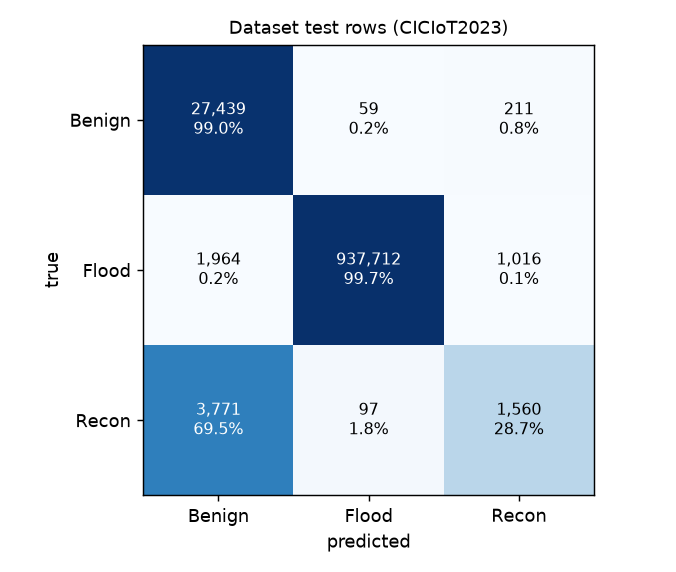
\includegraphics[width=0.5\linewidth]{images/cm_dataset_test.png}
\caption{Deployed model, confusion matrix on the CICIoT2023 test split.}
\end{figure}

\subsection{Training on the full dataset (100\%) instead of the 20\% sample}

Same recipe, same 14 features, all 4,546,831 kept rows (our rows split by time).

\begin{center}
\begin{tabular}{lcccccc}
\toprule
Training share & Macro-F1 & Binary F1 & Recon recall & Size & Train & Predict \\
\midrule
\dep 20\% (deployed recipe) & 0.760 & 0.997 & 0.291 & 918 KB & 7 s & 0.10 ms \\
100\% & 0.759 & 0.997 & 0.290 & 810 KB & 33 s & 0.07 ms \\
\bottomrule
\end{tabular}
\end{center}

\textbf{Finding:} five times more data gives the same scores; the 20\% sample is enough. (The 20\% row is a retrain
for this comparison; the deployed file scores 0.760 / 974 KB.)

% =====================================================================================================
\section{Objectives 4 and 5: live testbed and dashboard}

Real Raspberry Pi 4, 3 NodeMCU sensors, attacks from the laptop and from the NodeMCU bots (17 November, final
model; IPS on):

\begin{center}
\small\setlength{\tabcolsep}{4pt}
\begin{tabular}{llll}
\toprule
Attack & Alert & Conf. & Top-3 SHAP reasons \\
\midrule
SYN flood & DoS flood & 0.96 & Min, Std, ack\_flag\_number \\
UDP flood & DoS flood & 1.00 & Protocol Type, Min, UDP \\
ICMP flood & DoS flood & 1.00 & ICMP, Min, ack\_flag\_number \\
ACK flood & DoS flood & 0.98 & Min, Max, Std \\
PSH-ACK flood & DoS flood & 1.00 & psh\_flag\_number, Min, Max \\
RST-FIN flood & DoS flood & 1.00 & fin\_flag\_number, Min, rst\_flag\_number \\
Port scan & Recon (model + rule) & 0.99 / 1.00 & AVG, Tot size, Max \\
Version scan & Recon & 0.99 & AVG, Tot size, Max \\
MQTT brute force & BruteForce (rule) & 1.00 & refused MQTT logins \\
Bot DDoS (TCP, UDP) & DDoS (3 senders) & 0.96--1.00 & all 3 quarantined \\
\bottomrule
\end{tabular}
\end{center}

Every attack was detected and blocked; \textbf{no false alarms} on the 3 NodeMCUs. ARP spoofing could not be
tested on the college Wi-Fi: the access point rewrites spoofed ARP replies before they reach the gateway (verified
with tcpdump on the Pi). Dashboard: every alert with its top-3 SHAP features, the traffic, the sensors, and the
active blocks with IPS on/off and release controls.

% =====================================================================================================
\section{Open items}

\begin{center}
\begin{tabularx}{\linewidth}{P{5.2cm}L}
\toprule
Item & Status / next step \\
\midrule
RQ2 benchmark of all compressed models \emph{on the Pi} & script ready (\file{pi/benchmark/rq2\_benchmark.py},
about 2 minutes); laptop numbers reported above \\
Energy per 1,000 inferences & needs a USB power meter (the script has an energy mode) \\
Throughput measured on its own & derived from the latency so far; the benchmark script measures it \\
ESP32 nodes & NodeMCU (ESP8266) used: same family, same role \\
6-page IEEE paper & to be written from these results \\
\bottomrule
\end{tabularx}
\end{center}

\end{document}
